\documentclass[tikz]{standalone}
\input{common/tikzBase}
\usetikzlibrary{patterns,arrows.meta}
\newsavebox{\heapOverflowInObjCode}
\tikzset{
    stackBox/.style={very thick},
    onStack/.style={thick},
    frameOne/.style={fill=blue!15},
    frameTwo/.style={fill=red!15},
    markLine/.style={blue!50!black},
    markLineB/.style={red!90!black},
    hiLine/.style={red!90!black},
}
\begin{document}
\begin{lrbox}{\heapOverflowInObjCode}
\begin{lstlisting}
struct foo {
    char buffer[100];
    void (*func_ptr)(void);
};
\end{lstlisting}
\end{lrbox}

\setSlide{1}
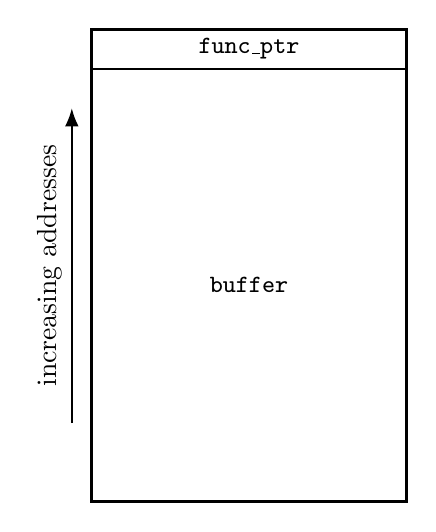
\begin{tikzpicture}
\draw[stackBox] (0, 0) rectangle (4, -6);
\draw[thick,-Latex] (-.25,-5) -- (-.25, -1) node [midway, above, sloped] {increasing addresses};
\draw[onStack] (0, -0.5) rectangle (4, -6) node[midway,font=\small] {\texttt{buffer}};
\draw[onStack] (0, -0) rectangle (4, -0.5) node[midway,font=\small] {\texttt{func\_ptr}};
\end{tikzpicture}

\end{document}
